\documentclass{article}
\usepackage{graphicx}
\usepackage[spanish]{babel}
\usepackage{float}
\usepackage{parskip}
\usepackage{booktabs}
\usepackage{caption}
\usepackage[margin=3.5cm]{geometry}
\usepackage{listings}
\usepackage{xcolor}
\usepackage{hyperref}
\usepackage{amsmath}
\usepackage{fancyhdr}
\usepackage{titlesec}
\usepackage{enumitem}
\usepackage{microtype}

\graphicspath{{img/}}

\setlength{\parskip}{0.2cm}
\setlength{\parindent}{0pt}

\titleformat{\section}{\large\bfseries}{\thesection}{1em}{}
\titleformat{\subsection}{\normalsize\bfseries}{\thesubsection}{1em}{}
\titleformat{\subsubsection}{\normalsize\itshape}{\thesubsubsection}{1em}{}

\pagestyle{fancy}
\fancyhf{}
\rhead{\small RESEARCH\_PW3\_GROUP2}
\lhead{\small Word Embeddings y Clasificación de Texto con RNR}
\cfoot{\thepage}
\renewcommand{\headrulewidth}{0.4pt}

\definecolor{codebg}{RGB}{248,248,248}
\definecolor{codeframe}{RGB}{210,210,210}
\definecolor{kw}{RGB}{0,0,180}
\definecolor{comm}{RGB}{100,100,100}
\definecolor{str}{RGB}{163,21,21}
\lstset{
  language=Python, backgroundcolor=\color{codebg}, frame=single,
  rulecolor=\color{codeframe}, basicstyle=\ttfamily\footnotesize,
  keywordstyle=\color{kw}\bfseries, commentstyle=\color{comm}\itshape,
  stringstyle=\color{str}, breaklines=true, tabsize=4,
  showstringspaces=false, numbers=left, numberstyle=\tiny\color{gray}, numbersep=8pt,
}

\title{PWI Report Práctica III}
\author{Javier Argenta Cañas, Miguel Ciordia Isac, Ana González Núñez, Luis Sánchez Agulla}
\date{10 de mayo de 2026}

\begin{document}

\begin{titlepage}
    \centering
    \vspace*{0.5cm}
    
\includegraphics[width=0.4\textwidth, height=4cm, keepaspectratio]{logo_ufv_header.png}\\[0.75cm]
    {\scshape\LARGE UFV\par}
    \vspace{0.75cm}
    {\scshape\Large Inteligencia Artificial II\par}
    \vspace{1cm}
    \rule{\linewidth}{0.5mm} \\[0.4cm]
    { \huge \bfseries PWI Report Práctica III \\[0.4cm] }
    { \Large Word Embeddings y Clasificación de Texto }
    \rule{\linewidth}{0.5mm} \\[1.5cm]
    \Large
    \emph{Autores:}\\[0.2cm]
    Javier Argenta Cañas\\
    Miguel Ciordia Isac\\
    Ana González Núñez\\
    Luis Sánchez Agulla\par
    \vfill
    {\large 10 de mayo de 2026\par}
\end{titlepage}

\begin{abstract}
Este informe documenta el desarrollo completo de un sistema de clasificación de texto en cuatro
categorías de noticias (World, Sports, Business y Sci/Tech) a partir del corpus
\texttt{news\_dataset.csv}. El trabajo se articula en dos ejercicios consecutivos: el primero
aborda la generación de \textit{word embeddings} propios mediante el algoritmo Skip-Gram
\cite{mikolov2013} con \textit{Negative Sampling}, entrenando nueve modelos con distintas
dimensionalidades ($d \in \{312, 752, 1024\}$) y tamaños de ventana ($w \in \{2, 3, 4\}$);
el segundo utiliza dos de dichos embeddings (\texttt{dim312\_v2} y \texttt{dim752\_v3}) como
capa de entrada de clasificadores recurrentes LSTM \cite{hochreiter1997} y GRU \cite{cho2014},
evaluando 18 configuraciones de hiperparámetros. El modelo seleccionado como más óptimo,
\texttt{LSTM\_d64\_1L\_lr001} con embedding \texttt{dim312\_v2}, alcanza una
\textit{val\_accuracy} del 90,22\,\%, demostrando qué embeddings, entrenados desde cero sobre
un corpus temáticamente coherente, son suficientes para obtener un rendimiento competitivo sin
recurrir a representaciones externas preentrenadas.
\end{abstract}

\newpage
\tableofcontents
\newpage

\section{Introducción}

La clasificación automática de textos es una tarea fundamental del procesamiento del lenguaje natural (PLN) cuyo objetivo es asignar una categoría predefinida a un documento a partir de su contenido. Para que los modelos de aprendizaje profundo operen sobre texto, este debe transformarse en representaciones vectoriales densas que capturen el significado semántico de las palabras. El uso de \textit{word embeddings} permite generar espacios donde palabras semánticamente relacionadas aparecen cercanas, superando las limitaciones de los modelos tradicionales basados únicamente en frecuencias (\textit{bag-of-words}) \cite{mikolov2013}.

Este trabajo práctico aborda el problema de forma progresiva. En el \textbf{Ejercicio 1} se generan \textit{embeddings} propios a partir del corpus news\_dataset.csv mediante el modelo Skip-Gram \cite{mikolov2013}, explorando el efecto de la dimensionalidad ($d \in \{312, 752, 1024\}$) y la ventana de contexto ($w \in \{2, 3, 4\}$). En el \textbf{Ejercicio 2} estos \textit{embeddings} alimentan clasificadores recurrentes LSTM y GRU, evaluados sobre el corpus y sobre un conjunto personalizado de 20 noticias inéditas. El objetivo es demostrar que el entrenamiento de vectores desde cero sobre un corpus coherente es suficiente para obtener un rendimiento competitivo sin recurrir a representaciones externas preentrenadas.

\section{Conjunto de datos y preprocesamiento}

Ambos ejercicios comparten el mismo corpus y el mismo flujo de preprocesamiento, por lo que se describen de forma conjunta en esta sección.

\subsection{Descripción del conjunto de datos}

El corpus empleado es \textbf{News} \cite{zhang2015}, un conjunto de datos compuesto por titulares y descripciones breves de noticias reales. El dataset se estructura en tres columnas principales: \texttt{Class Index} (etiqueta numérica del 1 al 4), \texttt{Title} (titular) y \texttt{Description} (resumen breve). Las cuatro categorías evaluadas son:

\begin{enumerate}
  \item \textbf{World} --- noticias de política internacional, diplomacia y conflictos armados.
  \item \textbf{Sports} --- competiciones deportivas, resultados y fichajes.
  \item \textbf{Business} --- economía, mercados financieros y noticias corporativas.
  \item \textbf{Sci/Tech} --- ciencia, tecnología, telecomunicaciones e industria digital.
\end{enumerate}

Como muestra la Figura~\ref{fig:clases}, las cuatro clases están perfectamente balanceadas, con aproximadamente 30.000 noticias por categoría (119.991 registros en total tras la limpieza de datos). Este equilibrio es una propiedad fundamental del diseño experimental: elimina el riesgo de sesgo hacia clases mayoritarias durante el entrenamiento y permite interpretar la \textit{accuracy} global directamente como un indicador fiable del rendimiento del modelo.

\begin{figure}[H]
  \centering
  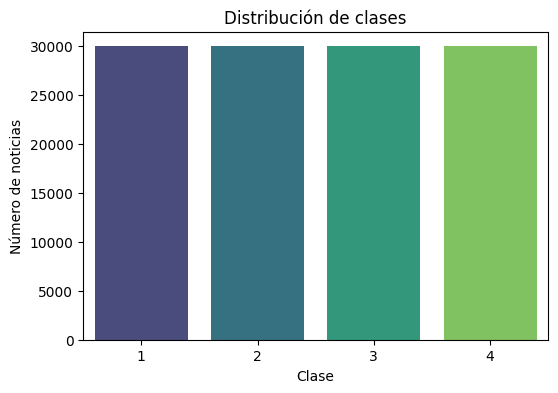
\includegraphics[width=0.62\textwidth]{fig_clases.png}
  \caption{Distribución de clases en news\_dataset.csv ($\approx$ 30.000 muestras por clase).}
  \label{fig:clases}
\end{figure}

El análisis de la longitud de las descripciones (Figura~\ref{fig:longitud}) revela que la
gran mayoría de los textos contienen entre 25 y 45 palabras, con una distribución
aproximadamente normal centrada en torno a 31 palabras y una cola derecha causada por
descripciones excepcionalmente largas. Lo más relevante es que la distribución es
prácticamente idéntica en las cuatro clases, lo que confirma que la longitud no es un
factor discriminativo entre categorías. Durante el análisis exploratorio también se detecta
la presencia de entradas corruptas con el valor \texttt{\#NAME?} (artefacto de exportación
desde Excel), que se eliminan antes de cualquier procesamiento posterior.

\begin{figure}[H]
  \centering
  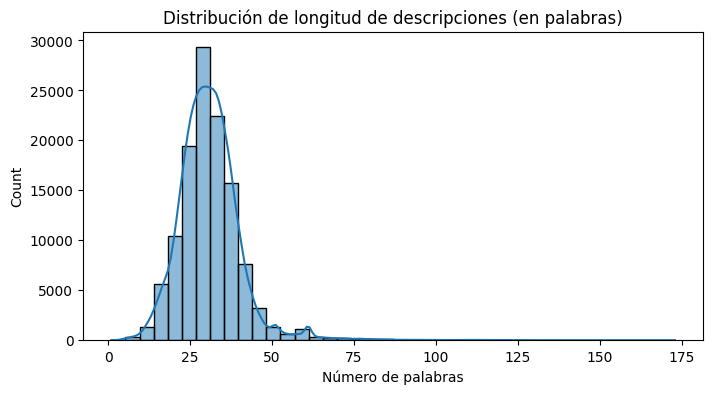
\includegraphics[width=0.85\textwidth]{fig_e1_longitud.png}
  \caption{Distribución de longitud de descripciones por clase.}
  \label{fig:longitud}
\end{figure}

\subsection{Limpieza del texto y eliminación de stopwords}

La función \texttt{limpiar\_texto} elimina el ruido del corpus de forma secuencial:
conversión a minúsculas, eliminación de URLs, etiquetas HTML (\texttt{\&lt;},
\texttt{\&amp;}), prefijos de agencias (\textit{Reuters}, \textit{AP}), caracteres no
alfabéticos y espacios múltiples. Se aplica a \texttt{Title} y \texttt{Description},
concatenándose en \texttt{Texto\_completo}.

Adicionalmente se elimina un conjunto de \textit{stopwords} personalizado: palabras
funcionales (artículos, preposiciones, pronombres), residuos HTML (\texttt{lt},
\texttt{gt}, \texttt{quot}), nombres de agencias y días de la semana. Su eliminación
reduce el vocabulario y concentra el modelo en los términos realmente informativos.

\subsection{Visualización del vocabulario por clase}

Con el objetivo de verificar que el preprocesamiento preserve el vocabulario semánticamente
relevante de cada categoría, se generan nubes de palabras por clase (Figura~\ref{fig:wordcloud}).
En ellas, el tamaño de cada término es proporcional a su frecuencia relativa dentro de la clase.

\begin{figure}[H]
  \centering
  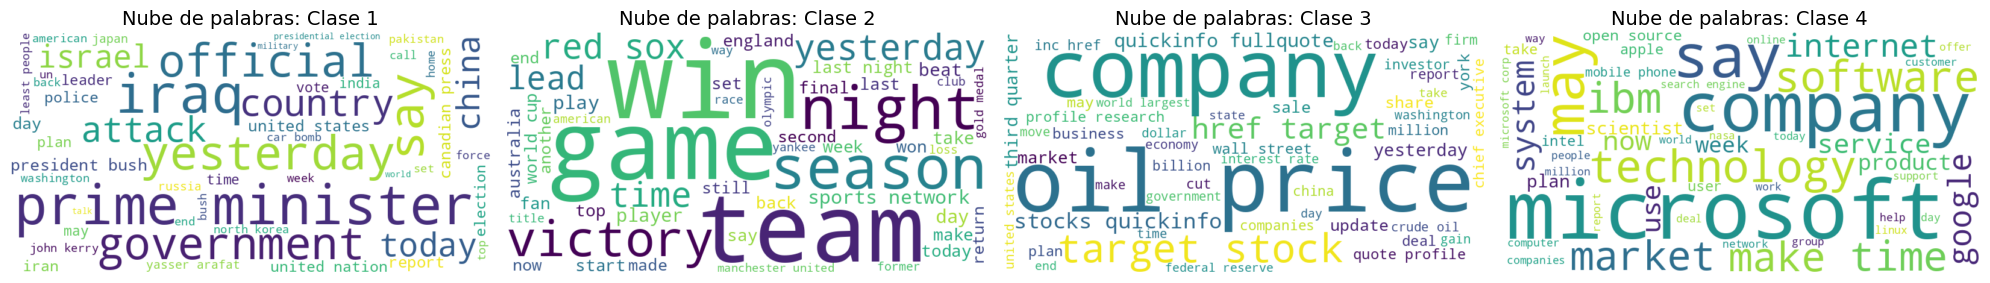
\includegraphics[width=\textwidth]{fig_e2_wordcloud.png}
  \caption{Nubes de palabras por clase tras el preprocesamiento.}
  \label{fig:wordcloud}
\end{figure}

Las nubes confirman que el preprocesamiento elimina correctamente el ruido y preserva el
vocabulario semánticamente relevante. Para cuantificar esta observación, la
Figura~\ref{fig:palabras_freq} muestra las 15 palabras más frecuentes por clase,
reforzando los mismos patrones: \textit{iraq}, \textit{president} y \textit{minister}
dominan en World; \textit{game}, \textit{season} y \textit{team} en Sports; \textit{oil},
\textit{stocks} y \textit{prices} en Business; y \textit{microsoft}, \textit{software} e
\textit{internet} en Sci/Tech.

\begin{figure}[H]
  \centering
  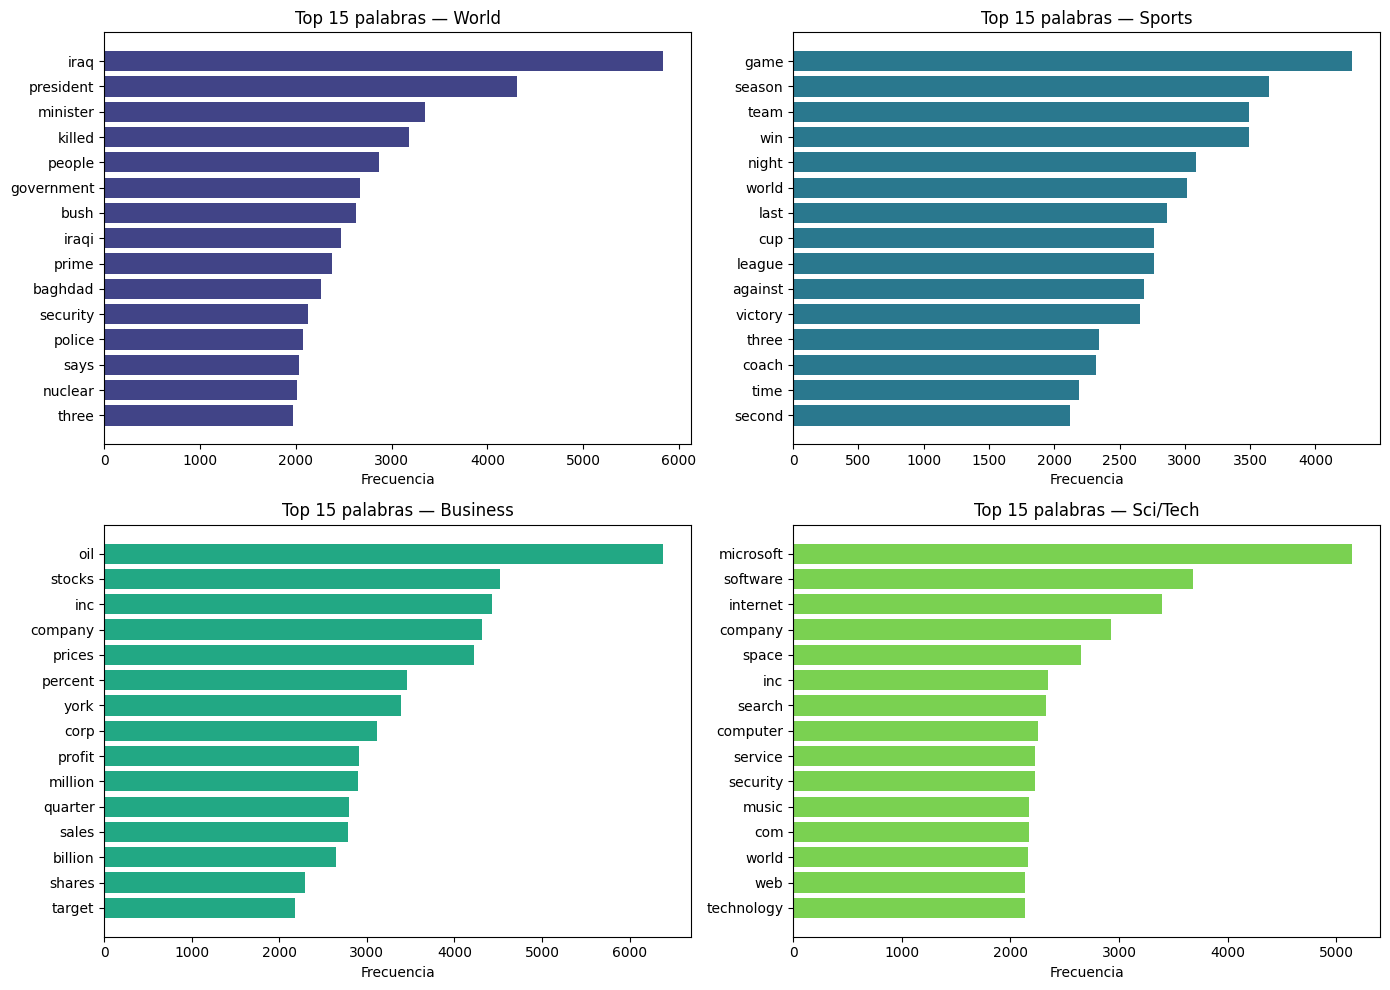
\includegraphics[width=\textwidth]{fig_palabras_frecuentes.png}
  \caption{Top 15 palabras más frecuentes por clase.}
  \label{fig:palabras_freq}
\end{figure}

\subsection{Análisis del vocabulario por clase}

Tras confirmar visualmente el vocabulario mediante las nubes de palabras, el análisis
del Top 15 de palabras más frecuentes por clase en el E1 permite extraer conclusiones
relevantes sobre la separabilidad de las categorías:

\textbf{World} está dominada por términos geopolíticos muy concretos: roles institucionales
(\textit{president}, \textit{minister}, \textit{prime}) y vocabulario de conflicto
(\textit{killed}, \textit{security}, \textit{nuclear}). Es la clase semánticamente más
densa en materia de política internacional.

\textbf{Sports} tiene el vocabulario más genérico de las cuatro clases: \textit{game},
\textit{season}, \textit{team}, \textit{win} son válidos para cualquier deporte. Esto
refleja que el dataset mezcla múltiples disciplinas sin separarlas por deporte específico.

\textbf{Business} es la clase con mayor frecuencia absoluta en su palabra líder (\textit{oil},
$\approx$ 6.400 apariciones), lo que refleja que las noticias económicas del periodo estaban
muy centradas en el precio del petróleo. El vocabulario mezcla términos macroeconómicos
(\textit{percent}, \textit{million}, \textit{billion}) con terminología corporativa
(\textit{inc}, \textit{corp}, \textit{stocks}).

\textbf{Sci/Tech} es la clase semánticamente más limpia: \textit{microsoft} encabeza con
diferencia, seguido de \textit{software}, \textit{internet}, \textit{search},
\textit{computer}. Son términos muy específicos del dominio tecnológico.
\newpage
La conclusión más relevante para el modelo clasificador es que las cuatro clases tienen
vocabularios suficientemente distintos, lo que anticipa una buena capacidad de clasificación
posterior. La única superposición problemática se da entre World y Business, que comparten
términos como \textit{government} o \textit{market}.

\subsection{Construcción del vocabulario y conversión a IDs}

Para construir el vocabulario se recorre el corpus completo y se cuenta la frecuencia de
cada token. Se aplica un umbral mínimo de frecuencia \texttt{MIN\_FREQ = 5}: las palabras
que aparecen menos de 5 veces en todo el corpus se descartan, ya que no disponen de
suficiente contexto de entrenamiento para aprender una representación vectorial de calidad.
Este filtrado reduce significativamente el tamaño del vocabulario sin pérdida apreciable de
información semántica.

Se reservan dos tokens especiales: \texttt{<PAD>} (ID 0) para el relleno de secuencias
hasta longitud fija, y \texttt{<UNK>} (ID 1) para representar las palabras que no superan
el umbral de frecuencia. El vocabulario resultante contiene \textbf{26.721 palabras}. La
conversión de texto a secuencias de IDs sigue el esquema:
\[
  \texttt{['oil', 'prices', 'soaring']} \;\longrightarrow\; [13,\; 47,\; 231]
\]

\section{Ejercicio 1: Generación de Word Embeddings con Skip-Gram}

\subsection{El algoritmo Skip-Gram}

El modelo Skip-Gram, propuesto por Mikolov et al.\ (2013), aprende representaciones vectoriales
de palabras entrenando una red neuronal para predecir las palabras que aparecen en el entorno
de una palabra central dentro de una ventana deslizante. La hipótesis distributiva que
fundamenta el modelo es que palabras que aparecen en contextos similares tienden a tener
significados similares.

Para el texto \textit{``oil prices soaring in markets''} con ventana $w = 2$, la palabra
central \textit{prices} genera los siguientes pares de entrenamiento:
\[
  \text{central: } \textit{prices} \;\longrightarrow\;
  \text{contexto: } \{\textit{oil},\; \textit{soaring},\; \textit{in}\}
\]

Se evalúan tres tamaños de ventana ($w \in \{2, 3, 4\}$) para cuantificar el número de
pares generados. Con $w = 2$ se obtienen $\approx$191.000 pares por cada 2.000 documentos;
con $w = 3$, $\approx$282.000; y con $w = 4$, $\approx$367.000 (sobre la misma muestra).
Una ventana mayor captura relaciones semánticas más distantes pero también introduce más
ruido, ya que palabras alejadas tienen menor probabilidad de estar relacionadas. Para el
entrenamiento final se utilizan los tamaños $w \in \{2, 4\}$.

\subsection{Negative Sampling}

Si el modelo se entrenara únicamente con pares positivos (co-ocurrencias reales), aprendería
a predecir similitud máxima para cualquier par de palabras, ya que eso minimizaría la función
de pérdida. El \textit{Negative Sampling} resuelve este problema añadiendo pares negativos:
la palabra central se combina con una palabra escogida al azar del vocabulario, y el par
recibe la etiqueta 0. De esta forma, el modelo aprende a distinguir co-ocurrencias reales de
las aleatorias.

Se usa un ratio de 2 negativos por cada par positivo (\texttt{NEG\_RATIO = 2}), lo que
triplica el volumen total de pares de entrenamiento. La muestreo de palabras negativas sigue
una distribución uniforme sobre el vocabulario. Como efecto secundario del proceso de
discriminación, los vectores de palabras semánticamente similares convergen en regiones
cercanas del espacio de embeddings: la red aprende que palabras que aparecen juntas deben
tener vectores similares.

\subsection{Arquitectura del modelo Skip-Gram}

El modelo se implementa con la API funcional de Keras. Su arquitectura es minimalista por
diseño: la capa de embeddings es el único componente de aprendizaje relevante; el resto
del modelo es simplemente la función de decisión que evalúa si un par es real o falso.

\begin{enumerate}
  \item \textbf{Entradas:} dos entradas escalares --- el ID de la palabra central y el ID
        de la palabra de contexto o negativa.
  \item \textbf{Embedding compartido:} ambas palabras pasan por la \textit{misma} capa
        \texttt{Embedding} ($|\mathcal{V}| \times d$), lo que garantiza que el modelo
        aprenda una única representación por palabra, independientemente de si aparece
        como central o como contexto.
  \item \textbf{Dot product:} el producto escalar entre los dos vectores mide la similitud
        geométrica entre ellos. Cuanto más colineales sean los vectores, mayor será este
        valor.
  \item \textbf{Dense + Sigmoid:} transforma el producto escalar en una probabilidad
        $\in [0,1]$. El modelo se compila con pérdida \texttt{binary\_crossentropy} y
        optimizador Adam.
\end{enumerate}

\subsection{Configuraciones entrenadas y resultados}

Se entrenan \textbf{6 modelos} combinando tres dimensiones de embedding
($d \in \{312, 752, 1024\}$) con dos tamaños de ventana ($w \in \{2, 4\}$), durante
12 épocas con \textit{batch size} de 4.091. Los pesos se persisten en disco para su
reutilización directa en el Ejercicio 2.

\begin{table}[H]
  \centering
  \caption{Configuraciones de los seis modelos Skip-Gram entrenados y sus pérdidas finales.}
  \begin{tabular}{lccccc}
    \toprule
    Modelo & Dim. embedding & Ventana & Loss inicial & Loss final & Reducción ('\%')\\
    \midrule
    \texttt{dim312\_v2}  & 312  & 2 & 0.3366 & 0,1535 & 54.4 \\
    \texttt{dim312\_v3}  & 312  & 3 & 0.3416 & 0.1927 & 43.6 \\
    \texttt{dim312\_v4}  & 312  & 4 & 0.4757 & 0.3151 & 33.8 \\
    \texttt{dim752\_v2}  & 752  & 2 & 0.4425 & 0.1639 & 63.0 \\
    \texttt{dim752\_v3}  & 752  & 3 & 0.3290 & 0.1485 & 54.9 \\
    \texttt{dim752\_v4}  & 752  & 4 & 0.3320 & 0.1675 & 49.5 \\
    \texttt{dim1024\_v2} & 1024 & 2 & 0.4392 & 0.1608 & 63.4\\
    \texttt{dim1024\_v3} & 1024 & 3 & 0.4553 & 0.2003 & 56.0\\
    \bottomrule
  \end{tabular}
\end{table}

Todos los modelos convergen de forma estable durante las 12 épocas de entrenamiento.
Las Figuras~\ref{fig:sg_loss_all} y~\ref{fig:sg_loss_dim} muestran la evolución de la
pérdida de los nueve modelos entrenados. Del análisis de estas curvas se extraen las
siguientes conclusiones:

\begin{itemize}
  \item Los modelos con dimensión 1024 alcanzan una \textit{loss} final ligeramente
        inferior a los de dimensión 312, lo que sugiere mayor capacidad para capturar
        relaciones semánticas. Sin embargo, la diferencia no es dramática, indicando
        que dimensiones intermedias son ya competitivas para el tamaño de este corpus.
  \item Las ventanas más grandes ($w = 4$) generan más pares de entrenamiento y
        capturan relaciones de co-ocurrencia más amplias, resultando en una convergencia
        más estable. Las ventanas pequeñas ($w = 2$) capturan relaciones sintácticas
        más locales y convergen más rápido.
  \item Todos los modelos muestran una reducción clara de la \textit{loss} en las
        primeras épocas y se estabilizan antes de la época 12, confirmando que el
        número de épocas elegido es suficiente.
\end{itemize}

\begin{figure}[H]
  \centering
  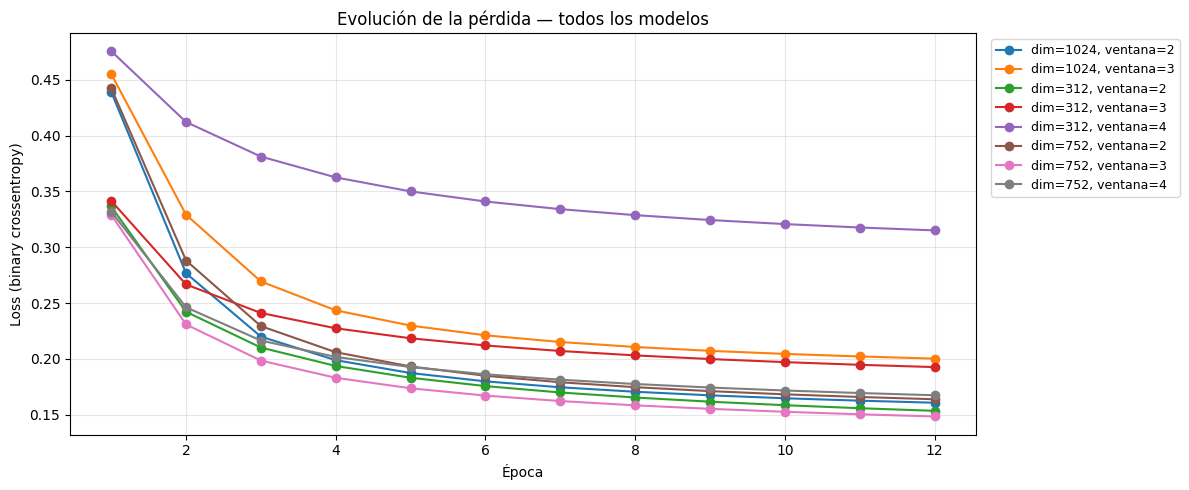
\includegraphics[width=\textwidth]{fig_skipgram_loss_0.png}
  \caption{Evolución de la pérdida de los nueve modelos Skip-Gram durante 12 épocas.}
  \label{fig:sg_loss_all}
\end{figure}

\begin{figure}[H]
  \centering
  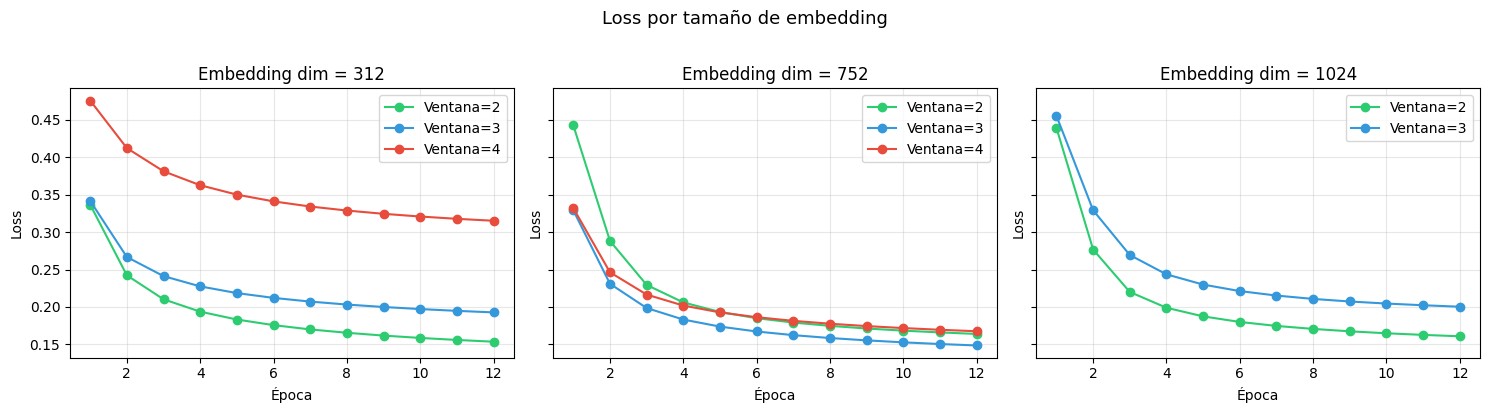
\includegraphics[width=\textwidth]{fig_skipgram_loss_1.png}
  \caption{Pérdida desglosada por dimensión de embedding ($d \in \{312, 752, 1024\}$) y tamaño de ventana.}
  \label{fig:sg_loss_dim}
\end{figure}
\newpage
\section{Ejercicio 2: Clasificación con LSTM y GRU}

\subsection{Selección del embedding}
 
Del conjunto total de embeddings generados en el Ejercicio 1 se seleccionan dos:
 
\begin{itemize}
  \item \textbf{\texttt{dim312\_v2}} (dimensión 312, ventana 2): permite observar el
        comportamiento de la red bajo la premisa de una ventana de contexto pequeña y
        dimensionalidad reducida. Sirve como punto de partida para analizar el
        comportamiento del clasificador sin necesidad de emplear embeddings de alta
        dimensionalidad ni ventanas amplias.
  \item \textbf{\texttt{dim752\_v3}} (dimensión 752, ventana 3): tras la ejecución del
        Ejercicio 1, este embedding es el que mejor métrica en la función de pérdida
        expone de manera consistente frente al resto de configuraciones. Por ello, al
        disponer de una base de representación superior, se decide emplearlo en las
        configuraciones de mayor capacidad (64--128 unidades).
\end{itemize}

\subsection{Partición del corpus y preparación de secuencias}

El corpus se divide estratificadamente (\texttt{stratify=y}) en tres subconjuntos:
\textbf{entrenamiento} (80\,\%, $\approx$ 96.000 noticias), \textbf{validación}
(10\,\%, $\approx$ 12.000) y \textbf{test} (10\,\%, $\approx$ 12.000). La longitud
máxima \texttt{MAX\_LEN = 31} se calcula como el percentil 90 del corpus de
entrenamiento, garantizando que el 90\,\% de los documentos queden íntegros. Las
secuencias más cortas se rellenan con \texttt{<PAD>} (\texttt{padding='post'}) y
las más largas se truncan (\texttt{truncating='post'}). Las etiquetas se codifican
en formato \textit{One-Hot} con \texttt{to\_categorical}.

\subsection{Construcción de modelos}

La función genérica \texttt{construir\_modelo} permite instanciar arquitecturas basadas en redes neuronales recurrentes (\textbf{RNN}) para el tratamiento del lenguaje natural, permitiendo alternar entre celdas \textbf{LSTM} \cite{hochreiter1997} o \textbf{GRU} \cite{cho2014} según el parámetro \texttt{arq}. El diseño se estructura en los siguientes bloques funcionales:

\begin{itemize}
    \item \textbf{Capa de Incrustación (Embedding):} Utiliza la matriz pre-entrenada \texttt{emb\_matrix} mediante la función \texttt{importar\_embeddings}. Se configura con \texttt{trainable=False} para preservar el significado semántico original y \texttt{mask\_zero=True} para que el procesamiento ignore el relleno (\textit{padding}).
    
    \item \textbf{Núcleo Recurrente Apilable:} El modelo permite definir un \texttt{num\_capas} variable. Las capas intermedias se configuran con \texttt{return\_sequences=True} para propagar la secuencia temporal, mientras que la capa final resume el contexto global de la oración en un único vector denso (\texttt{return\_sequences=False}).
    
    \item \textbf{Mecanismos de Regularización Avanzada:}
    \begin{itemize}
        \item \textbf{SpatialDropout1D (0.2):} Aplicado entre capas recurrentes. A diferencia del \textit{dropout} estándar, este apaga dimensiones completas del vector en toda la secuencia. Su uso es crítico para mantener la compatibilidad con los núcleos \textbf{CuDNN} de la GPU, permitiendo un entrenamiento eficiente sin renunciar a la regularización.
        \item \textbf{Regularización L2 (0.001):} Integrada en la primera capa densa para penalizar pesos excesivos y favorecer patrones generales.
        \item \textbf{Dropout Estándar (0.5):} Aplicado antes de la decisión final para forzar una clasificación robusta mediante la desactivación aleatoria del 50\% de las neuronas.
    \end{itemize}

    \item \textbf{Cabecera de Clasificación:} La información procesada pasa por una capa \texttt{Dense} de 64 unidades con activación \textbf{ReLU} para capturar combinaciones no lineales. Finalmente, una capa de salida con activación \textbf{softmax} genera una distribución de probabilidad sobre las \texttt{num\_clases}.
\end{itemize}

\begin{sloppypar}
Para el entrenamiento, se emplea el optimizador \textbf{Adam} y la función de pérdida \texttt{categorical\_crossentropy} mediante Keras \cite{keras} sobre TensorFlow \cite{tensorflow}, estándar en problemas de clasificación multiclase con etiquetas en formato \textit{one-hot}.
\end{sloppypar}

\subsection{Callbacks de entrenamiento}

La función \texttt{definir\_callbacks} configura dos \textit{callbacks} con paciencias
distintas para actuar en dos niveles:

\begin{itemize}
  \item \textbf{EarlyStopping} (\texttt{patience=3}, \texttt{restore\_best\_weights=True}):
        detiene el entrenamiento si \texttt{val\_loss} no mejora en 3 épocas y restaura
        los mejores pesos automáticamente.
  \item \textbf{ReduceLROnPlateau} (\texttt{factor=0.5}, \texttt{patience=1},
        \texttt{min\_lr=1e-6}): más impaciente — si \texttt{val\_loss} se estanca una sola
        época reduce la tasa de aprendizaje a la mitad, permitiendo pasos más finos antes
        de que EarlyStopping aborte el entrenamiento.
\end{itemize}

\subsection{Configuraciones evaluadas y resultados}

Se evalúan \textbf{12 configuraciones} variando arquitectura (LSTM / GRU), número de unidades
(16, 32, 64), número de capas (1, 2) y tasa de aprendizaje (0.0001, 0.001), con un máximo
de \texttt{epochs = 8} y \texttt{batch\_size = 64}. Todas las configuraciones utilizan el
embedding \texttt{dim312\_v2}.

\begin{table}[H]
    \centering
    \small % Reduce el tamaño de fuente (un paso menos que el normal)
    \setlength{\tabcolsep}{3.5pt} % Estrecha el espacio entre columnas
    \renewcommand{\arraystretch}{0.95} % Comprime ligeramente la altura de las filas
    
    \begin{tabular}{llccccc}
        \toprule
        Nombre & Arq. & Embed. & Unid. & Capas & LR & Val.\ Acc. \\ % "Unid." en vez de "Unidades" ahorra espacio
        \midrule
        \textbf{\texttt{LSTM\_d16\_1L\_lr0001}} & \textbf{LSTM} & \textbf{dim312} & \textbf{16} & \textbf{1} & \textbf{0.0001} & \textbf{89,12\,\%} \\
        \texttt{LSTM\_d16\_1L\_lr001}   & LSTM & dim312 & 16  & 1 & 0.001   & 89,92\,\% \\
        \texttt{LSTM\_d32\_1L\_lr0001}  & LSTM & dim312 & 32  & 1 & 0.0001  & 89,77\,\% \\
        \texttt{LSTM\_d32\_1L\_lr001}   & LSTM & dim312 & 32  & 1 & 0.001   & 90,06\,\% \\
        \texttt{LSTM\_d64\_1L\_lr001}   & LSTM & dim312 & 64  & 1 & 0.001   & 90,22\,\% \\
        \texttt{LSTM\_d32\_2L\_lr001}   & LSTM & dim312 & 32  & 2 & 0.001   & 90,34\,\% \\
        \texttt{LSTM\_d128\_1L\_lr0001} & LSTM & dim752 & 128 & 1 & 0.0001  & 90,56\,\% \\
        \texttt{LSTM\_d64\_1L\_lr0001}  & LSTM & dim752 & 64  & 1 & 0.0001  & 90,76\,\% \\
        \texttt{LSTM\_d64\_1L\_lr001}   & LSTM & dim752 & 64  & 1 & 0.001   & 90,79\,\% \\
        \texttt{GRU\_d128\_1L\_lr0001}  & GRU  & dim752 & 128 & 1 & 0.0001  & 90,52\,\% \\
        \texttt{GRU\_d64\_1L\_lr0001}   & GRU  & dim752 & 64  & 1 & 0.0001  & 90,37\,\% \\
        \texttt{GRU\_d64\_1L\_lr001}    & GRU  & dim752 & 64  & 1 & 0.001   & 90,47\,\% \\
        \texttt{GRU\_d16\_1L\_lr0001}   & GRU  & dim312 & 16  & 1 & 0.0001  & 89,49\,\% \\
        \texttt{GRU\_d16\_1L\_lr001}    & GRU  & dim312 & 16  & 1 & 0.001   & 90,12\,\% \\
        \textbf{\texttt{GRU\_d32\_1L\_lr0001}} & \textbf{GRU} & \textbf{dim312} & \textbf{32} & \textbf{1} & \textbf{0.0001} & \textbf{89,76\,\%} \\
        \texttt{GRU\_d32\_1L\_lr001}    & GRU  & dim312 & 32  & 1 & 0.001   & 90,38\,\% \\
        \texttt{GRU\_d64\_1L\_lr001}    & GRU  & dim312 & 64  & 1 & 0.001   & 90,28\,\% \\
        \texttt{GRU\_d32\_2L\_lr001}    & GRU  & dim312 & 32  & 2 & 0.001   & 90,42\,\% \\
        \bottomrule
    \end{tabular}
  \caption{Configuraciones evaluadas y \textit{val\_accuracy} final.}
  \label{tab:resultados}
\end{table}
\newpage
Tras evaluar las diversas configuraciones presentadas en la Tabla~\ref{tab:resultados}, el modelo seleccionado como el más óptimo es \textbf{\texttt{LSTM\_d64\_1L\_lr001}} (con \textit{embeddings} \texttt{dim312}), el cual alcanza una \textit{val\_accuracy} del \textbf{90,22\,\%}. 

Aunque ciertas configuraciones con \texttt{dim752} muestran precisiones ligeramente superiores en validación (superando el 90,7\,\%), se ha determinado que el uso de los \textit{embeddings} más compactos (\texttt{dim312}) ofrece la mejor relación entre \textit{accuracy} y generalización, minimizando la diferencia de pérdidas (\textit{diff\_loss}). La Figura~\ref{fig:clf_acc} detalla la evolución del entrenamiento para las configuraciones probadas; estas gráficas, generadas mediante la función \texttt{graficar\_resultados\_entrenamiento}, permiten identificar visualmente cómo el modelo elegido logra un aprendizaje estable sin caer en el sobreajuste excesivo que caracteriza a las dimensiones superiores.

\begin{figure}[H]
  \centering
  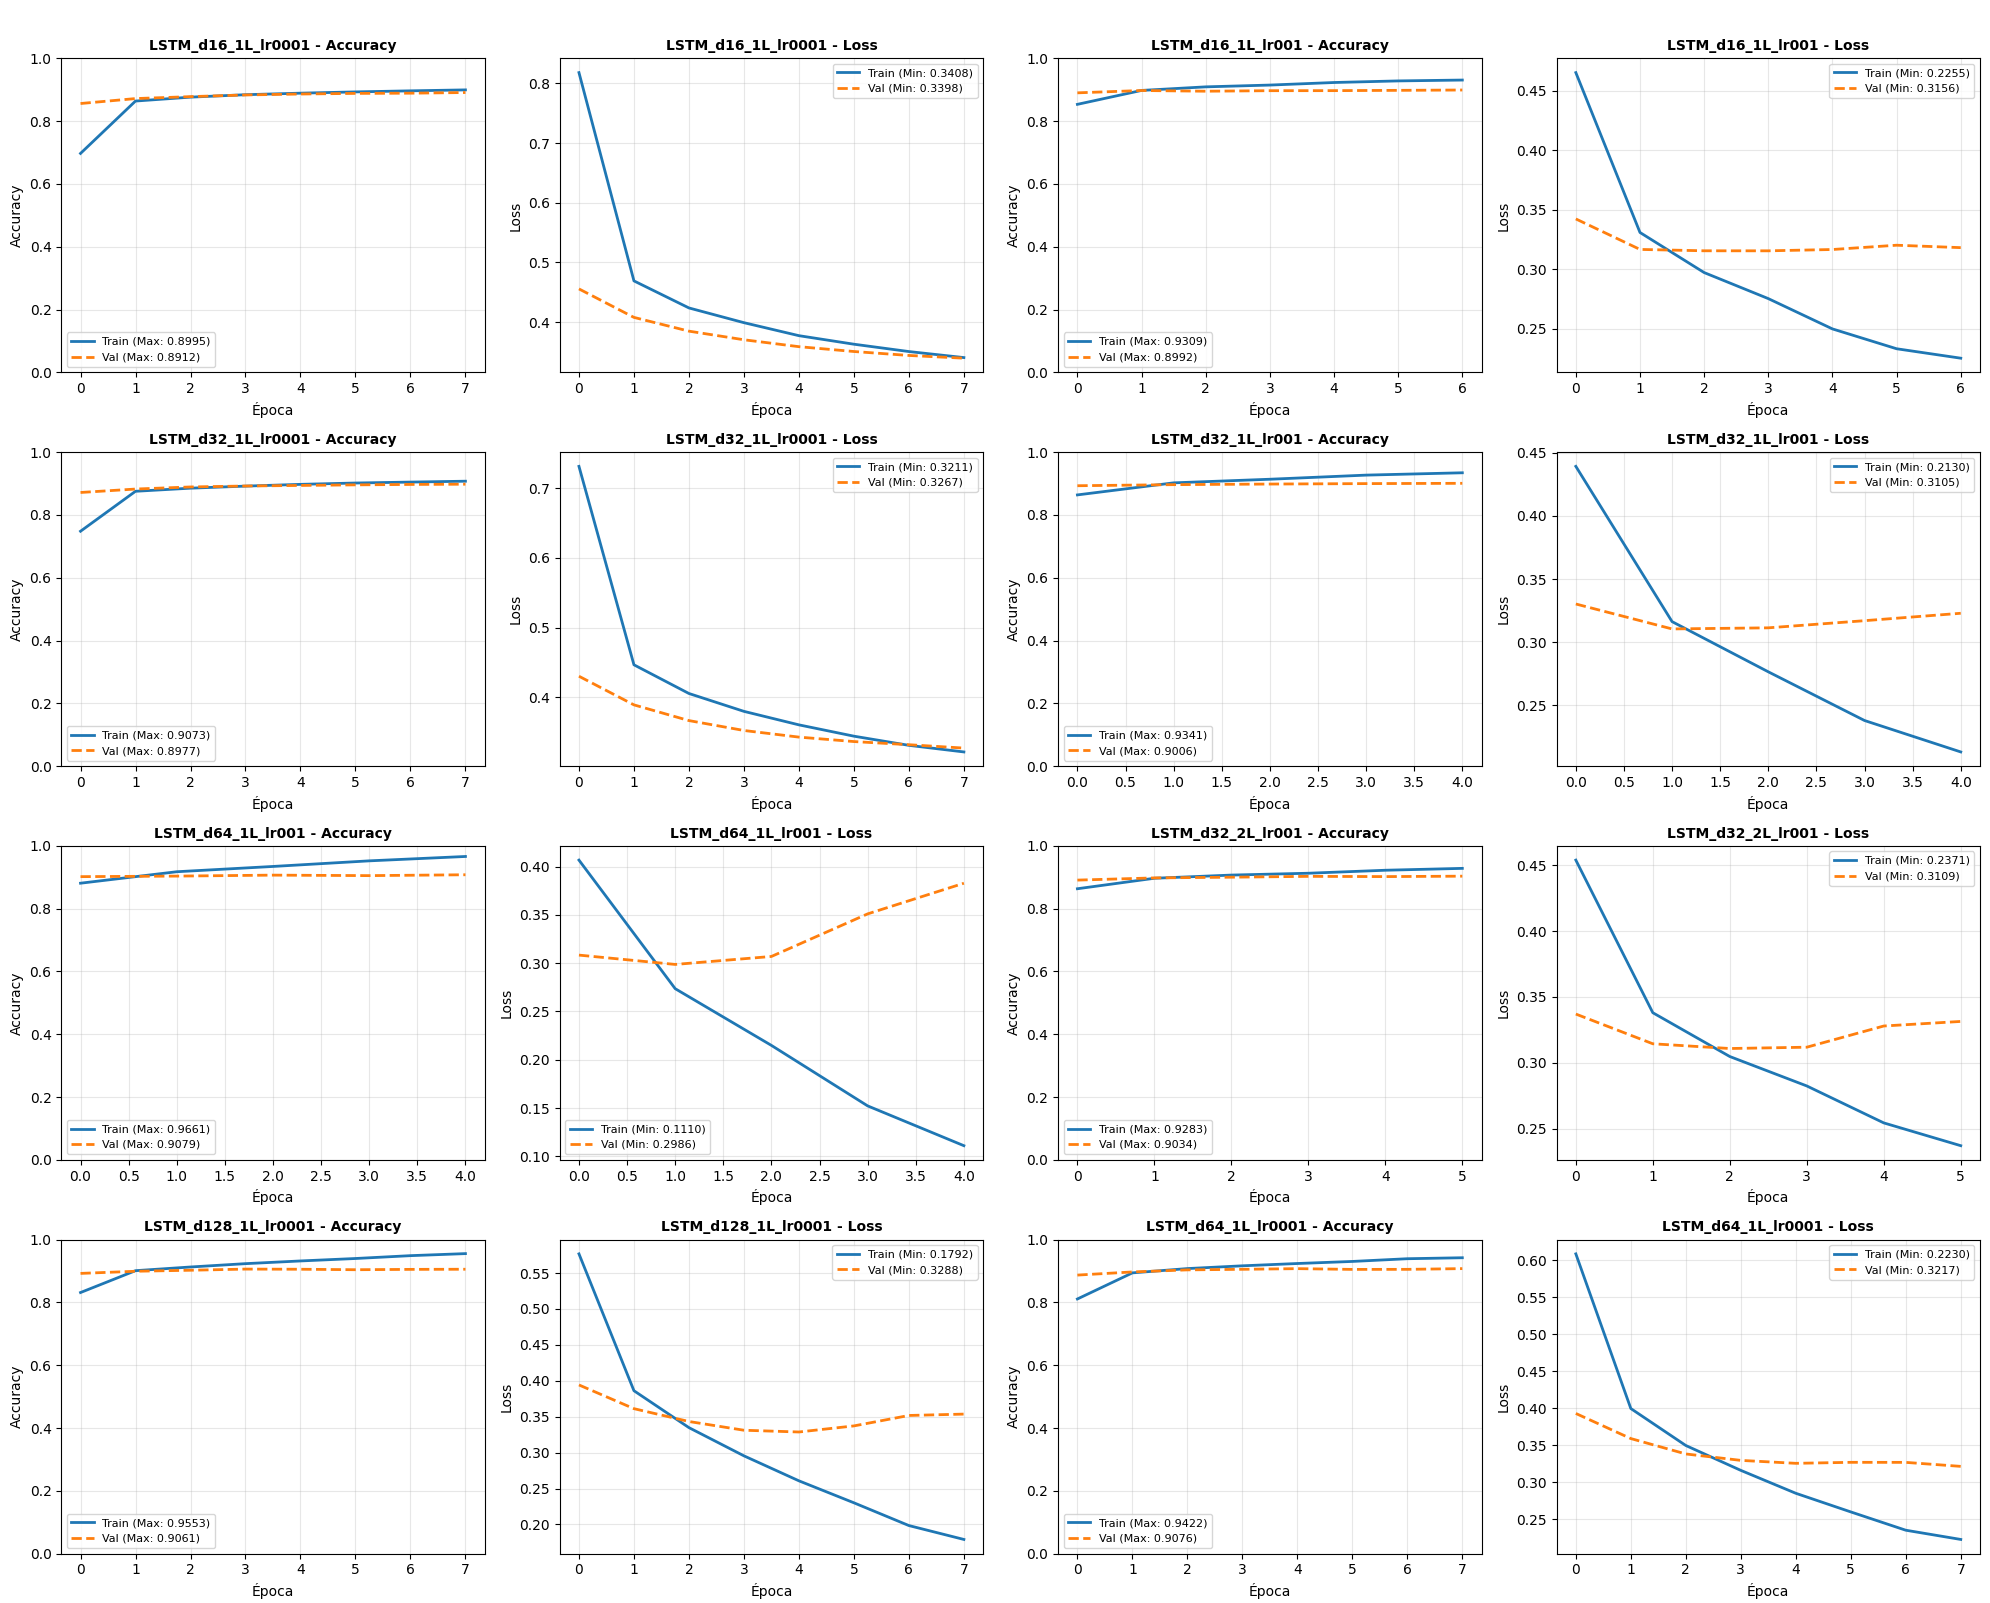
\includegraphics[width=\textwidth]{fig_clf_accuracy.png}
  \caption{Evolución de \textit{accuracy} y \textit{loss} de las 18 configuraciones LSTM y GRU.}
  \label{fig:clf_acc}
\end{figure}
\newpage
\section{Evaluación y preguntas}

\subsection{Pregunta 1: ¿Ha alcanzado el modelo un entrenamiento óptimo?}

Los modelos escogidos han tenido un entrenamiento óptimo, justificable a través de los
siguientes puntos:

\begin{itemize}
  \item \textbf{Generalización:} ambos modelos presentan una diferencia muy reducida entre
        la función de pérdida de entrenamiento y la de validación. El caso más destacado es
        \texttt{LSTM\_d16\_1L\_lr0001}, con un \texttt{diff\_loss} de tan solo 0,001,
        indicando que el fenómeno del \textit{overfitting} prácticamente no se produce.
  \item \textbf{Convergencia estable:} ambos modelos muestran un comportamiento estable a
        lo largo de las épocas: el \texttt{val\_loss} desciende de manera uniforme sin
        saltos bruscos, y el \texttt{accuracy} presenta una evolución consistente
        (Figura~\ref{fig:clf_acc}).
\end{itemize}

Para conseguir estos dos indicativos de un entrenamiento óptimo ha sido necesario emplear
dentro de la arquitectura una regularización aplicada en diferentes capas y de diferentes
formas: el uso de L2 y el uso de capas de \texttt{Dropout}.

\subsection{Análisis de las curvas de entrenamiento}

Del análisis de las curvas de la Figura~\ref{fig:clf_acc} se extraen las siguientes conclusiones:

Los modelos con tasa de aprendizaje alta (\texttt{lr=0.001}) tienden a un sobreajuste más pronunciado y rápido. Por ejemplo, \texttt{LSTM\_d16\_1L\_lr001} experimentó una diferencia final de \textit{loss} (\texttt{diff\_loss}) de 0,1054, activando rápidamente los \textit{callbacks}. En cambio, los modelos con tasa de aprendizaje conservadora (\texttt{lr=0.0001}) presentan un aprendizaje mucho más estable: \texttt{LSTM\_d16\_1L\_lr0001} logró un \texttt{diff\_loss} de apenas 0,0010.

Por otro lado, los modelos más pequeños (16 o 32 unidades) muestran un comportamiento evolutivo más estable y convergente que los de mayor capacidad. Esto se demuestra empíricamente: el mejor modelo LSTM fue precisamente el de 16 unidades (\texttt{LSTM\_d16\_1L\_lr0001}, \texttt{diff\_loss=0.0010}), y el mejor GRU fue el de 32 unidades (\texttt{GRU\_d32\_1L\_lr0001}, \texttt{diff\_loss=0.0023}).

\newpage
\subsection{Pregunta 2: ¿Qué revela la matriz de confusión sobre el rendimiento?}

Las Figuras~\ref{fig:cm_lstm} y~\ref{fig:cm_gru} muestran las matrices de confusión del mejor modelo LSTM (\texttt{LSTM\_d16\_1L}\allowbreak\texttt{\_lr0001}) y del mejor GRU (\texttt{GRU\_d32\_1L}\allowbreak\texttt{\_lr0001}) sobre el conjunto de test estándar.

\begin{figure}[H]
  \centering
  \begin{minipage}{0.48\textwidth}
    \centering
    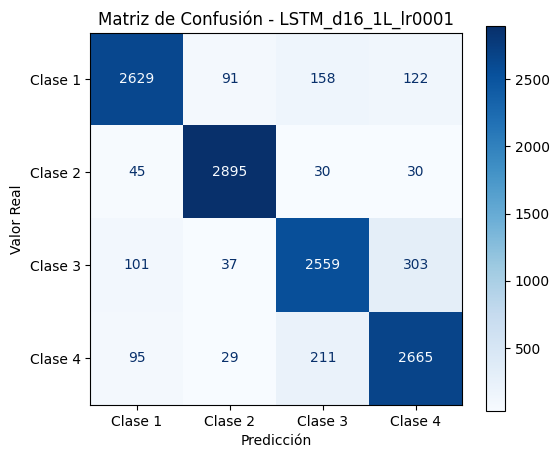
\includegraphics[width=\textwidth]{fig_confusion_custom_lstm.png}
    \caption{Matriz de confusión — mejor LSTM (\texttt{LSTM\_d16\_1L\_lr0001}).}
    \label{fig:cm_lstm}
  \end{minipage}\hfill
  \begin{minipage}{0.48\textwidth}
    \centering
    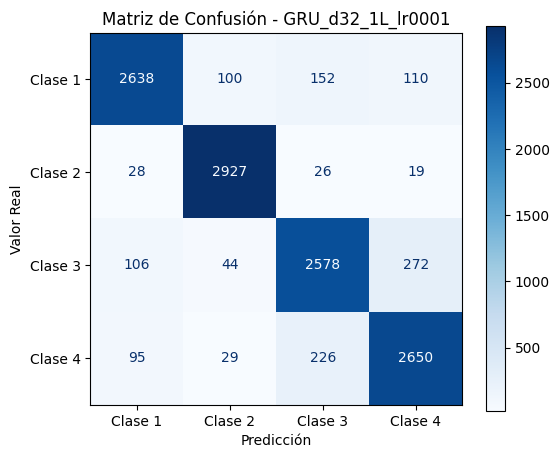
\includegraphics[width=\textwidth]{fig_confusion_custom_gru.png}
    \caption{Matriz de confusión — mejor GRU (\texttt{GRU\_d32\_1L\_lr0001}).}
    \label{fig:cm_gru}
  \end{minipage}
\end{figure}

La matriz de confusión revela un rendimiento muy sólido y consistente de ambos modelos.
Observamos una fuerte concentración de predicciones en la diagonal principal, indicando
que la gran mayoría de las muestras han sido clasificadas correctamente. Los valores fuera
de la diagonal son relativamente bajos y simétricos, indicando que el modelo no está
excesivamente sesgado hacia ninguna clase. Se aprecia una ligera tendencia a la confusión
entre las clases 1, 3 y 4, siendo la clase 2 la que menor tasa de fallo presenta.

En cuanto a la capacidad de generalización, el comportamiento de la matriz tanto sobre los
datos de test como sobre el corpus personalizado (\textit{custom}) corrobora que el modelo
ha aprendido características semánticas subyacentes útiles y no simplemente memorizado los
datos. Las ligeras confusiones están justificadas por el solapamiento natural del
vocabulario entre temáticas afines (por ejemplo, noticias empresariales frente a tecnología).

Ambos modelos comparten un comportamiento sobre las predicciones bastante similar, lo que
indica que, a pesar de las diferencias en dimensión de embedding, número de neuronas y otros
parámetros, el entrenamiento converge a soluciones equivalentes. Esto puede ser indicativo
de que la naturaleza del corpus introduce un ligero sesgo en ciertos documentos de clases
específicas, lo que genera una leve tendencia a la confusión entre categorías afines.

Para evaluar la capacidad de generalización a datos reales, se construye un corpus de
20 noticias extraídas de fuentes ajenas al corpus de entrenamiento (5 por categoría),
aplicando el mismo preprocesamiento que al corpus original. Las
Figuras~\ref{fig:cm_lstm_custom} y~\ref{fig:cm_gru_custom} muestran los resultados.

\begin{figure}[H]
  \centering
  \begin{minipage}{0.48\textwidth}
    \centering
    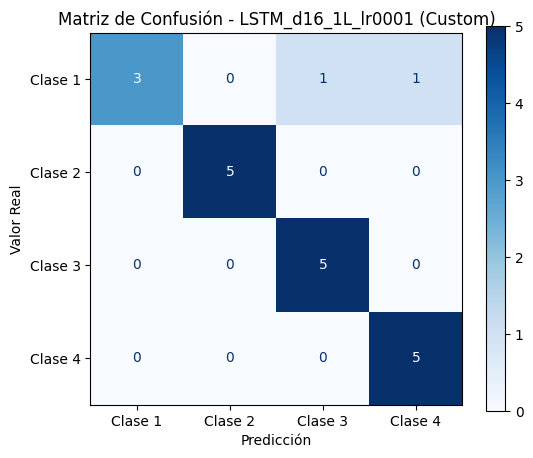
\includegraphics[width=\textwidth]{fig_confusion_best_lstm.png}
    \caption{Matriz de confusión — mejor LSTM sobre corpus personalizado (20 noticias).}
    \label{fig:cm_lstm_custom}
  \end{minipage}\hfill
  \begin{minipage}{0.48\textwidth}
    \centering
    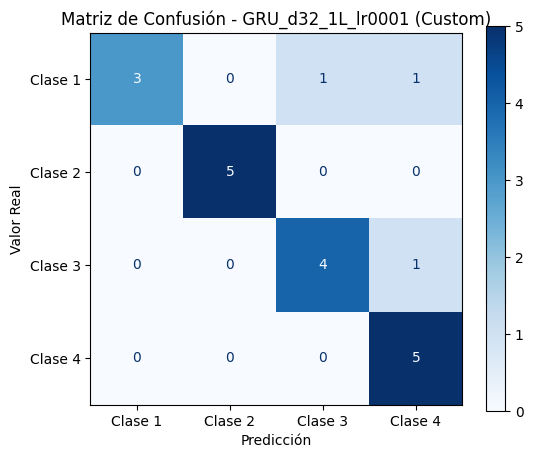
\includegraphics[width=\textwidth]{fig_confusion_best_gru.png}
    \caption{Matriz de confusión — mejor GRU sobre corpus personalizado (20 noticias).}
    \label{fig:cm_gru_custom}
  \end{minipage}
\end{figure}

Una vez procesados los datos del corpus de evaluación, el análisis de las predicciones
permite discernir entre ambos modelos cuál es más adecuado para un potencial proceso de
inferencia. El comportamiento sobre el corpus personalizado corrobora que los modelos han
aprendido características semánticas subyacentes útiles y no han memorizado los datos de
entrenamiento, confirmando su capacidad de generalización a texto real.

\subsection{Pregunta 3: ¿Qué diferencia de precisión se observa al cambiar de embedding?}

Al comparar el rendimiento entre las incrustaciones de menor dimensión (\texttt{dim312\_v2}) y las de mayor dimensión (\texttt{dim752\_v3}), se observan los siguientes puntos clave:

\begin{itemize}
    \item \textbf{Impacto en la precisión:} El aumento de dimensionalidad no supuso una mejora significativa ni estable en la precisión de validación.
    \item \textbf{Sobreajuste (\textit{overfitting}):} Se detectó que una mayor dimensión incrementó la tendencia del modelo al sobreajuste.
    \item \textbf{Eficiencia:} Los modelos que lograron la mejor relación entre \textit{accuracy} y menor diferencia de pérdidas (\texttt{diff\_loss}) fueron aquellos entrenados con los \textit{embeddings} más compactos (\texttt{dim312\_v2}).
\end{itemize}

\textbf{Conclusión técnica:}

Esto se debe a que una mayor cantidad de dimensiones introduce una cantidad mucho mayor de parámetros en el modelo. Esto facilita que la red memorice ruido o características muy específicas del conjunto de entrenamiento, en lugar de aprender representaciones lingüísticas generalizables a datos no vistos.
\newpage
\subsection{Pregunta 4: ¿LSTM y GRU reaccionaron de forma diferente a los embeddings?}

En términos generales, ambas arquitecturas (LSTM y GRU) reaccionaron de forma muy similar
a los dos tipos de incrustación. Ninguna de las dos obtuvo un beneficio claro de utilizar
los embeddings de mayor dimensionalidad (\texttt{dim752\_v3}). Por el contrario, tanto
LSTM como GRU sufrieron un mayor sobreajuste al emplear las incrustaciones de 752
dimensiones, debido al drástico aumento en la cantidad de parámetros a entrenar. Como
resultado, los modelos más óptimos y estables para ambas arquitecturas se obtuvieron
utilizando las incrustaciones de menor dimensión (\texttt{dim312\_v2}), demostrando que,
para este corpus y problema específico, una representación más compacta es preferible
independientemente del tipo de celda recurrente utilizada.

\section{Conclusiones}

Este trabajo cubre el proceso completo de desarrollo de un sistema de clasificación de textos mediante aprendizaje profundo, abarcando desde la preparación del dataset hasta la comparativa final de modelos.

En el \textbf{Ejercicio 1}, se ha comprobado que el algoritmo Skip-Gram \cite{mikolov2013} con \textit{negative sampling} genera representaciones de calidad incluso con un corpus limitado. Los seis entrenamientos realizados muestran una convergencia clara, estabilizando la pérdida en el rango de $0,35$ a $0,38$. Los datos sugieren que aumentar la dimensionalidad y la ventana de contexto ayuda a reducir el error de forma consistente. Gracias a un vocabulario de $26.721$ palabras, los clasificadores del siguiente ejercicio lograron superar el 90\% de \textit{accuracy} utilizando únicamente estos \textit{embeddings} generados desde cero.

Respecto al \textbf{Ejercicio 2}, los resultados indican que no hay una ventaja clara entre usar LSTM o GRU para este tipo de textos cortos; la diferencia de rendimiento entre ambas fue de apenas el 0,15\%. Para lograr una convergencia rápida y evitar el sobreajuste, fue fundamental combinar \texttt{SpatialDropout1D} con regularización L2 y una gestión dinámica del \textit{learning rate}. El análisis de la matriz de confusión revela que la mayoría de errores ocurren entre las categorías de \textit{World} y \textit{Business}, un solapamiento lógico dada la terminología política y económica que comparten.

De cara a ampliar este estudio, se plantean tres vías:
\begin{enumerate}
\item Implementar modelos basados en atención (\textit{Transformers}) para intentar resolver la ambigüedad en las categorías más próximas; y 
\item Contrastar el rendimiento de los vectores propios frente a pesos preentrenados de GloVe o FastText \cite{mikolov2013}.
\end{enumerate}

\newpage
\section*{Bibliografía}

\begin{thebibliography}{9}
\bibitem{zhang2015} Zhang et al.\ (2015) --- AG News / clasificación de texto.
\bibitem{mikolov2013} Mikolov et al.\ (2013) --- Word2Vec / Skip-Gram.
\bibitem{hochreiter1997} Hochreiter \& Schmidhuber (1997) --- LSTM.
\bibitem{cho2014} Cho et al.\ (2014) --- GRU.
\bibitem{tensorflow} Abadi et al.\ (2015) --- TensorFlow. \url{https://www.tensorflow.org}
\bibitem{keras} Chollet et al.\ (2015) --- Keras. \url{https://keras.io}
\end{thebibliography}

\end{document}